\documentclass[12pt]{article}
\usepackage{graphicx}
\usepackage{listings}
\usepackage{setspace}
\usepackage{hyperref}
\usepackage{fancyhdr}
\usepackage{enumitem}

\usepackage{amsmath,amssymb,amsthm}
\usepackage{xcolor}
\usepackage{mdframed}

%--- environments ---
\newtheorem{theorem}{Theorem}[section]
\newtheorem{corollary}[theorem]{Corollary} % shares numbering with Theorem
\newtheorem{lemma}[theorem]{Lemma}
\newtheorem{proposition}[theorem]{Proposition}

%--- Boxed styling for theorems/corollaries/etc. ---
\surroundwithmdframed[
  skipabove=8pt, skipbelow=8pt,
  linewidth=1pt,
  linecolor=blue!60!black,
  backgroundcolor=blue!5,
  innertopmargin=6pt, innerbottommargin=6pt,
  innerleftmargin=6pt, innerrightmargin=6pt
]{theorem}

\surroundwithmdframed[
  skipabove=8pt, skipbelow=8pt,
  linewidth=1pt,
  linecolor=green!50!black,
  backgroundcolor=green!5,
  innertopmargin=6pt, innerbottommargin=6pt,
  innerleftmargin=6pt, innerrightmargin=6pt
]{corollary}

\usepackage{float}
\usepackage{geometry}
\geometry{margin=1in}
\usepackage{tikz}
\usetikzlibrary{arrows,automata}
\pagestyle{fancy}
\fancyhf{}
\rhead{Caleb K.}
\lhead{Non-Comparison Sorting Algorithm}
\cfoot{\thepage}

\title{Proof-of-Concept for a Non-Comparison, Non-Iterative Sorting Algorithm Based On Combinatoric Properties}
\author{Caleb K.}
\date{\today}

\setlength{\parskip}{10pt} 
\begin{document}

\maketitle

\begin{abstract}
This paper presents a novel sorting algorithm that does not rely on element comparisons or list iterations to sort elements, providing proofs and conjectures for specific test cases where this algorithm is effective and others where it may fail.
\end{abstract}

\section{Introduction}

Sorting algorithms are sets of rules and operations that can be applied to a list of values, allowing them to be arranged in order.

Common implementations of sorting algorithms, like Bubble Sort or Quick Sort, rely on element comparisons, directly comparing the numerical values of different elements and determining which is lower or greater. This allows a list of numbers to be arranged accordingly to approach a sorted state.

While non-comparison sorting algorithms exist, they may depend on list iteration. For example, Counting Sort loops through a pre-built list and iterates through it to count elements in the original list.

However, the algorithm we will define next will not depend on element comparison or list iteration to sort elements, except to check for when the list is sorted. For convenience, we will refer to it as numerical sorting in this paper.

\section{Numerical Sorting Algorithm Description}
Let $L$ be a list of integers that we want to sort in ascending order, where $|L|$ is the length of $L$.

Firstly, we will define a new operation called a shift as follows.

\subsection*{Shift Definition}

\begin{itemize}
    \item Take the first element $n = L[0]$.
    \item If $n < |L|$, shift $n$ forward by $n$ positions.
    \item Otherwise, move $n$ to the end of the list.
\end{itemize}

Formally, the shift can be described as the following.
\[
\text{shift}(L) = 
\begin{cases}
L[1:n+1] \| [L[0]] \| L[n+1:] & \text{if } n < |L|\\
L[1:] \| [L[0]] & \text{otherwise}
\end{cases}
\]

The algorithm repeats the shift operation until the list is sorted, which is verified by checking that all elements are in ascending order, after condition $n \geq |L|$ has been met and a shift has been performed.

\subsection*{Example Case}

{\setstretch{1.5}
Consider the list $L=[3,1,2,4]$, which we will sort with numerical sorting.

First, we will perform a shift, moving L[0] 3 elements forward, since $L[0]=3$.

This gives us $[1,2,4,3]$. Thus, we continue with the shift operations as follows.
}%

\subsubsection{Shift Operations}
\begin{enumerate}[start=0]
    \item $[3, 1, 2, 4]$ (original list)
    \item $[1, 2, 4, 3]$ (3 is shifted forward by 3 elements)
    \item $[2, 1, 4, 3]$ (1 is shifted forward by 1 element)
    \item $[1, 4, 2, 3]$ (3 is shifted forward by 3 elements)
    \item $[4, 1, 2, 3]$ (1 is shifted forward by 1 element)
    \item $[1, 2, 3, 4]$ ($4 \geq len(L)$, thus 4 is shifted to the back. Check triggered, list is sorted)
\end{enumerate}

To elaborate on the fifth shift, when $L[0]$ is 4, the condition of $n < |L|$ is not met because there are only three elements with a greater index than 4. This means that we cannot shift $L[0]$ 4 elements forward, and instead we will shift $L[0]$ to the back of the list, to $[1,2,3,4]$.

This additionally triggers a check to verify that the list is sorted, which it is. Thus, we have sorted the list [3, 1, 2, 4] using the algorithm and verified that it works for this arrangement.

However, to be clear, numerical sorting fails to sort a list in a finite number of shift operations in certain cases, which will be clarified later.

\subsection*{Python Implementation}
Below is a basic Python implementation of numerical sorting, following the algorithmic steps defined previously.

\begin{lstlisting}[language=Python]
#Function to check if list l is sorted.
def is_sorted(l):
    for i in range(len(l)-1):
        if l[i] > l[i+1]:
            return False
    return True

#Numerical sorting function, performing shifts until l is sorted.
def sort(l):
    s = len(l)
    while True:
        n = l[0]
        if n < s:
            l = l[1:n+1] + [n] + l[n+1:]
        else:
            l = l[1:] + [n]
            if is_sorted(l):
                return l
\end{lstlisting}

\section{Fail Cases}
The algorithm behind numerical sorting is defined only when any element $A_n \in \mathbb{Z}^+$ since shifting of negative numbers is undefined, and a shift of zero does not change the list order.

There are also certain cases in which numerical sorting fails, which are listed below.

\subsection{Duplicate Values}
Certain lists with duplicate values cannot be sorted if there exist undisplaceable numbers with positions unequal to their target positions.

This is because given the rules of the numerical sorting algorithm, where forward shift operations apply only to the first element, an element's index can only be increased if it is the first element and shifted. This new index will also be equal to $min(a,|L|-1)$, where $a$ is the value of the first element.

(If $a<|L|$, the element is shifted $a$ positions forward and has a new index of $0+a=a$. If $a \geq |L|$, the element is shifted to the back of the list and has a new index of $|L|$, where $|L|<0+a$ since $a \geq |L|$)

Consequently, the index of an element can only decrease if a front element shifts to a position greater than itself, freeing the first index and filling in a later index.

Let us continue to prove this statement, by considering a list $L = [a,...,b,...]$.

\subsubsection{Proof Of Stated Conditions Where An Element Decreases In Index During Numerical Sorting}

In numerical sorting, either a shift operation is performed, or a list is verified as sorted, keeping the list unchanged.

If the list remains unchanged, then the indices of its elements remain unchanged, and hence, elements never decrease in index.

Thus, we move on to consider shift operations.

Assuming that the shift of $a$ results in $a$ shifting to a position lower than $b$, where the index $a_i<b_i$, then the number of elements with a lower index than $b_i$ does not change.

This is because a shift operation removes the element at $i=0$ and splices the element at $i=min(a,|L|-1)$, as we have shown previously.

Thus, if $a$ shifts to a smaller index than $b$, then within the set of elements $S$ from index $0 \leq i < b$, the number of elements remains constant after the removal of $S[0]$ and the addition of the same element at $S[min(a,|L|-1)]$.

Hence, if an arbitrary first element $a$ in a list is shifted to a smaller position, and thus a smaller index than another arbitrary element $b$ in the same list, $b$ does not decrease in index.

However, if the shift of $a$ results in $a$ shifting to a position greater than $b$, where the index $a_i>b_i$, then the number of elements with a lower index than $b_i$ decreases by 1.

This is because within the set of elements $S$ from index $0 \leq i < b$, the removal of $S[0]$ decreases the number of elements by 1. The splicing of $S[0]$ does not add to the number of elements if $min(a,|L|-1)$ exceeds the given range of $S$ where $0 \leq i < b$.

Hence, if an arbitrary first element $a$ in a list is shifted to a greater position, and thus a greater index than another arbitrary element $b$ in the same list, $b$ decreases in index by 1.

Since any operation within the numerical sorting algorithm can be characterised into these three cases, one where the list is not altered due to the verification of sortedness, and another two where the first element $L[0]$ is shifted according to rules of where $L[0]<|L|$ and $L[0] \geq |L|$, then have proven that an element can only be displaced to the left and decreases in index if $L[0]$ shifts to a greater index than the element.

(This is because we have proven that the other two cases aside from the final case does not result in a given element being displaced to the left and decreasing in index)

Therefore, these results can be summarised as the following theorem.

\begin{theorem}
Given in a list $L$, there is an element $n$ with index $n_i$, $n_i$ increases only if $n_i=0$ and n is shifted. On the other hand, $n_i$ decreases only if $L[0]$ is shifted to an index greater than $n_i$, to $n_{i-1}$.
\end{theorem}

We will now continue to detail why certain lists where undisplaceable numbers exist cannot be sorted, and how duplicate values may contribute to this problem.

\subsubsection{Observation That Undisplaceable Elements Prevents List Sorting And Duplicate Values May Create Such Elements}

With the previous proofs, we can state that a list $L$ cannot be sorted using numerical sorting if there exists an element $k$ with index $k_i$ such that $k_i$ is not equal to its target position $T_k$, and the set of all numbers in previous positions contains no value greater or equal to $k_i$.

This is provable because we know that if $k_i<T_k$, it has to be displaced to the left so $k_i$ decreases to zero, enabling it to be shifted and increase in index to $min(k,|L|-1)$, where $k_i=T_k$ or $k$ can be displaced to the left and $k_i$ can decrease to $T_k$.

On the other hand, if $k_i>T_k$, it has to be displaced to the left so $k_i$ decreases to $T_k$.

Consider the unsorted list $[1,2,3,3,1]$, which results in the following repeating cycle.

\subsubsection{Shift Sequence}
\begin{enumerate}[start=0]
    \item $[1, 2, 3, 3, 1]$ (original list)
    \item $[2, 1, 3, 3, 1]$ (1 is shifted forward by 1 element)
    \item $[1, 3, 2, 3, 1]$ (2 is shifted forward by 2 elements)
    \item $[3, 1, 2, 3, 1]$ (1 is shifted forward by 1 element)
    \item $[1, 2, 3, 3, 1]$ (3 is shifted forward by 3 elements)
\end{enumerate}

After 4 operations, the sequence permutes back to the initial input $[1, 2, 3, 3, 1]$, without sorting once. Hence, $[1, 2, 3, 3, 1]$ is another list that cannot be sorted due to duplicate values.

This is also provable by inspection, because the element 1 at index 4 should be displaced to the left since $T_1<4$. $L[:4]$, the set of numbers before it, also contains no elements greater or equal to 4.

Hence, the last element 1 can never be displaced to its target position, and the list will not sort using numerical sorting.

We will summarise these results in the below theorem.

\begin{theorem}
 A list $L$ cannot be sorted using numerical sorting if there exists an element $k$ with index $k_i$ such that $k_i \neq T_k$, and $L[:k_i]$ contains no value greater or equal to $k_i$.
\end{theorem}

Since duplicates cannot contribute a value greater than the existing maximum, they cannot increase the greatest value of a subset. Hence, lists with duplicate values often result in this fail case.

However, it is important to note that this is not always the case, and that there are counterexamples such as the list $[4,1,1,2]$, in which the list sorts.

\subsubsection{Additional Note}
It is also critical to understand that some lists with duplicates such as $[2,1,1,4]$ will not be verified as sorted, even though it does converge to a sorted state. This is because the algorithm checks for sortedness only when a number $L[0]$ where $L[0]>|L|$ is shifted forward.

The logic for checking sortedness after this condition is because any element $L[0]$ where $L[0]<|L|$ in a given list $L$, will shift itself $L[0]$ elements forward. However, this means it will be the $L[0]+1$th element in the list, with an index of $L[0]$.

Therefore, if a list were to sort by ending at a shift operation where $L[0] < |L|$, the target index of $L[0]$, $T_{L[0]}$, would need to be $L[0]$. However, this is impossible for a list without duplicates.

This is because given the input domain of positive integer values, $T_{L[0]}$, when maximum, in a valid input list is $L[0]-1$, for a list that maximises this index by containing every consecutive number from 1 to $L[0]$.

If a list is missing any consecutive number, then $T_{L[0]}$ drops further from $L[0]$. Thus, a $T_{L[0]}=L[0]$ is unachievable given the shifting rules of $L[0]$ where $L[0]>|L|$. Therefore, the check is only considered when $L[0] \geq |L|$ for optimisation.

Below is an example to substantiate this proof.

\subsubsection{Example Proof}
Let an arbitrary list with no duplicates $L$ of length $|L|$ contain the number $k$, with all elements being positive integers in the domain $[1,\infty)$.

Let list $M$ be an arrangement of $L$ such that k is the first element, and it has k increasing elements in front of it that are all strictly less than k, followed by another arbitrary number of increasing elements. Let these elements also be positive integers in the domain $[1,\infty]$.

Thus, $M$ can be expressed as $[k, a_1, a_2, ..., a_k, a_{k+1},...]$ for some arbitrary elements $a_1, a_2, a_k, a_{k+1}$, and so on.

If a shift operation were to be applied to $M$, the resulting list could then be expressed as $M_1$, equal to $[a_1, a_2, ..., a_k, k, a_{k+1}, ...]$.

Since there are more than k elements in front of k, this shift operation follows the given algorithmic rules where $L[0] < |L|$. If we assume this rule can sort a list in one operation, this implies that list $L$ can be expressed as list $M_1$.

However, this leads to contradictions because there cannot be $k$ increasing positive integers with an index smaller than $k$ in $M_1$ that are strictly less than $k$. The maximum number of positive integers less than $k$ will have to be consecutive numbers. However, the $k$th element will still be equal to $k$, which violates the assumption that L has no duplicates.

Finally, if there are less than $k$ elements in front of $k$, such as in an arbitrary list $[k, a_1, a_2, ..., a_{k-1}]$, it violates the premise that the next shift operation follows the rules of a first element of value less than the length of the list.

Even in a case where there are more increasing elements after $a_{k-1}$, the index of $k$ in the shifted list is $k$, instead of the target index which decreases to $k-2$.

Therefore, by contradiction, shifting a list with no duplicates $L$ with an element $k = L[0]$ where $k$ is less than the length of its list $|L|$ cannot sort a list in one shift given the previously defined algorithmic rules.

The results of this proof can be summarised in the below theorem.

\begin{theorem}
A list $L$ with no duplicates can only be sorted in one shift if
$L[0] \geq |L|$, using numerical sorting.
\end{theorem}

\subsection{Alternating Subsequences Of Large Values}
Lists where there are alternating subsequences of large values will also not be sorted, because their alternating nature cannot be corrected by shifts.

To explain this, let us consider a list $L$ with four arbitrary elements $a, b, c, d$, where $a < b > c < d$, and $d > a$. Let us also assume that $a, b, c, d > |L|$.

Thus, defining $L = [a, b, c, d]$, let us attempt to perform shift operations on $L$ and observe if it sorts.

\subsubsection{Shift Sequence}
\begin{enumerate}[start=0]
    \item $[a, b, c, d]$ (original unsorted list)
    \item $[b, c, d, a]$ ($b > c$, so the list is not sorted)
    \item $[c, d, a, b]$ ($d > a$, so the list is not sorted)
    \item $[d, a, b, c]$ ($d > a$, so the list is not sorted)
    \item $[a, b, c, d]$ ($b > c$, so the list is not sorted and repeats)
\end{enumerate}

Given that elements $a, b, c, d > |L|$, the only possible change in these arrangements is to shift one to the back. However, since this only alters the inequality between only one set of adjacent elements (the new element at the back and the previous element at the back), it fails to resolve existing conflicts in inequality in the middle of the list.

However, this only applies if there are too many conflicting inequalities between elements that have greater value than the length of their lists.

Consider the counterexample $L = [10, 6, 9]$, with elements that have values all exceeding $|L|$, with a conflict in inequalities where $9 > 6 < 10$.

However, it is trivially easy to prove that $L$ is sortable, by performing a shift to permute it to $[6, 9, 10]$. But at the same time, the list $[10, 9, 6]$ fails to sort as it shifts from $[9, 6, 10]$, to $[6, 10, 9]$ and $[10, 9, 6]$ again.

This is because one also needs to consider the inequality between the first and last element in an alternating subsequence of values larger than $|L|$.

Listing out all the comparisons between adjacent elements in the previous examples moving from least index to largest index (including a comparison between the first and last element), we see that

For $[10, 6, 9]$, $10 > 6, 6 < 9, 9 < 10$, we can see it results in a two-length alternating subsequence that can be resolved by a single shift.

For $[9, 6, 10]$, $9 > 6, 6 < 10, 10 > 9$, however, we can see that it results in a three-length alternating subsequence that is not resolvable by a single shift.

\textbf{(Unfinished proof, work in progress! This will be updated in a future revision of this preprint.)}

\section{Combinatorial Analysis And Proof Of Sortable Sequences}
Although we have identified these fail cases that elaborate more on when numerical sorting fails, we have yet to prove that it will always sort a given list.

Although I am unable to prove this for every list that satisfies these fail cases, I am able to provide proofs that the following sequences are sortable.

\subsection{Index-bound Lists (1 to $|L|$)}
Let us first define a new category of lists known as \emph{index-bound} (IB) lists, that satisfy the following condition.

For any element $n$ in a index-bound list $L$, where $i$ is the index of $n$,
\begin{itemize}
    \item If $n < |L|$, then $0 \leq i \leq n$
\end{itemize}

Thus, we define any list that satisfies this condition as an \emph{index-bound} (IB) list, while a list that does not satisfy this condition is defined as a \emph{non-index-bound} (NIB) list.

To prove that index-bound lists that are arrangements of any consecutive list L from 1 to $|L|$ are sortable by numerical sorting, we can observe the interesting sequence that arises from attempting to sort lists of consecutive numbers from 1 to $|L|$.

Consider the sequence of shifts that result from sorting $L = [1,2,3]$ using numerical sorting. Note that the algorithm only verifies that a list is sorted if $L[0] \geq |L|$ and a shift is performed.

\subsubsection{Shift Sequence Of A Length-3 Consecutive List}
\begin{enumerate}[start=0]
    \item $[1, 2, 3]$ (original unsorted list)
    \item $[2, 1, 3]$
    \item $[1, 3, 2]$
    \item $[3, 1, 2]$
    \item $[1, 2, 3]$ (list sorted after 4 shifts)
\end{enumerate}

We can see that the sequence has cycled back to the same sorted consecutive list. We can also show this cycle occurs for consecutive lists of length 4 and 5.

\subsubsection{Shift Sequence Of A Length-4 Consecutive List}
\begin{enumerate}[start=0]
    \item $[1, 2, 3, 4]$ (original unsorted list)
    \item $[2, 1, 3, 4]$
    \item $[1, 3, 2, 4]$
    \item $[3, 1, 2, 4]$
    \item $[1, 2, 4, 3]$
    \item $[2, 1, 4, 3]$
    \item $[1, 4, 2, 3]$
    \item $[4, 1, 2, 3]$
    \item $[1, 2, 3, 4]$ (list sorted after 8 shifts)
\end{enumerate}

\subsubsection{Shift Sequence Of A Length-5 Consecutive List}
\begin{enumerate}[start=0]
    \item $[1, 2, 3, 4, 5]$ (original unsorted list)
    \item $[2, 1, 3, 4, 5]$
    \item $[1, 3, 2, 4, 5]$
    \item $[3, 1, 2, 4, 5]$
    \item $[1, 2, 4, 3, 5]$
    \item $[2, 1, 4, 3, 5]$
    \item $[1, 4, 2, 3, 5]$
    \item $[4, 1, 2, 3, 5]$
    \item $[1, 2, 3, 5, 4]$
    \item $[2, 1, 3, 5, 4]$
    \item $[1, 3, 2, 5, 4]$
    \item $[3, 1, 2, 5, 4]$
    \item $[1, 2, 5, 3, 4]$
    \item $[2, 1, 5, 3, 4]$
    \item $[1, 5, 2, 3, 4]$
    \item $[5, 1, 2, 3, 4]$
    \item $[1, 2, 3, 4, 5]$ (list sorted after 16 shifts)
\end{enumerate}

After observing the following sequences, we can see that lists of consecutive numbers L from 1 to $|L|$ cycle back after a certain number of shifts, permuting to index-bound lists at every step.

The pattern also seems to suggest that the number of shifts needed to sort a consecutive list L from 1 to $|L|$ using numerical sorting is equal to the formula $2^{|L|-1}$.

Suppose we prove that shift sequences of consecutive lists always cycle, and cover every index-bound list that can be expressed as an arrangement of a consecutive list L from 1 to $|L|$. In that case, we can prove that index-bound lists are always sortable using numerical sorting.

This is because any given index-bound list can then be found in the middle of this cycling sequence and thus will sort in a finite number of shifts.

First, we will prove that any consecutive list L from 1 to $|L|$ will always cycle, and after exactly $2^{|L|-1}$ shifts in numerical sorting.

\subsubsection{Inductive Proof Of Cycling In Consecutive List Numerical Sorting (1 to $|L|$)}

Let us demonstrate that this holds for any positive n greater than 2 using a proof by mathematical induction. We are not considering cases of lists length 1 because by definition such a list is already sorted because it has only one element.

Theorem:
A list of any consecutive integers starting from 1 with length n $(n > 1)$ will eventually sort itself again within $2^{|L|-1}$ shifts via numerical sorting.

Base Case:
Consider a list of length 2, with two consecutive integers, $[1,2]$. 

Then we can prove that it will sort itself again because it will undergo shifts to $[2,1]$ and back to $[1,2]$. It will also do this in $2^{n-1}$ shifts, equal to $2^{2-1}$.

Inductive Hypothesis:
Assume that a list of consecutive integers of arbitrary length k sorts itself again if enough shifts are applied to it, sorting within $2^{k-1}$ shifts.

Inductive Step:
Let a sortable list of length k be [1, … , k].

Then at some point, this list will undergo shifts to form the list $[k, 1, …, k-1]$. This is a conclusion derived from Theorem 3.1, since a sortable list L can only be sorted in one shift if $L[0] \geq |L|$, which only $k$ fulfills. It is also the only sequence where shifting $k$ to the last index results in an increasing sequence throughout the list, and sorting it.

Then, let a list of length $k+1$ be expressed as $[1, …, k-1, k, k+1]$

One can observe that if the list of length $k$ takes $2^{k-1}-1$ shifts to sort to $[k, 1, ..., k-1]$, then for a list of length $k+1$, it will permute to $[1, ..., k-1, k+1, k]$, taking $2^{k-1}$ shifts to permute to the given state.

This is because the addition of a new element at the end of the list does not change the number of shifts needed to displace $k$ to the first index, since if all numbers from 1 to $k-1$ were already smaller than $k$, it will still be smaller than $k+1$ in the list of length $k+1$, and follow the same algorithmic rules.

After $k$ is displaced to the front index, when it is shifted, it will be shifted behind $k-1$ and be the last element of the list since $k-1<k+1$, thus shifting $k$ elements forward.

Hence, after $2^{k-1}$ shifts, the list will permute to $[1, ..., k-1, k+1, k]$. 

Considering that within the set of elements from 1 to $k+1$, the numbers 1 to $k-1$ are still less than $k+1$, and given that we know that the list $[1, ..., k-1, k]$ managed to sort in $2^{k-1}$ shifts, then this shows that the previous elements will obey the same algorithmic steps, and $k+1$ will also be displaced to the front index in $2^{k-1}-1$ shifts.

Hence, after another $2^{k-1}-1$ shifts, the list has to permute to $[k+1, 1, ..., k-1, k]$. Then, since we know the elements from 1 to $k-1$ are increasing (given that the previous list was considered sorted and $k>k+1$), after another shift, the list will permute to $[1, ..., k-1, k, k+1]$ and sort itself again.

Finally, the number of shifts needed to sort the list $k+1$ can then be expressed as $2(2^{k-1}) = 2^{k+1-1} = 2^{|L|-1}$, if the new list were to be represented as L.

By the principle of mathematical induction, the theorem that index-bound lists cycle in $2^{|L|-1}$ holds for any index-bound list of any consecutive positive integers.

Now, given we have proved that consecutive lists from 1 to $|L|$ cycle through $2^{|L|-1}$ unique index-bound lists during sorting, we can prove that for any list L of length $|L|$, there are only $2^{|L|-1}$ possible arrangements of index-bound lists, to show that all index-bound lists are sortable.

We will summarise the results of this inductive proof below.

\begin{theorem}
A consecutive list L with unique elements from 1 to $|L|$ will cycle after $2^{|L|-1}$ shifts in numerical sort.
\end{theorem}

\subsubsection{Proof That Only $2^{|L|+1}$ Index-bound List Arrangements Exist For Any Given Consecutive List $L$ (1 to $|L|$)}

First, let us consider trying to construct every possible arrangement of a consecutive list L of length $|L|$ (from 1 to $|L|$) that is index-bound.

First, we take 1, which by the definition of index-bound lists, has to have an index i where $0 \leq i \leq 1$. This initial case gives us two potential arrangements, one where 1 is at the index zero and one where 1 is at the index one.

Now, consider taking the next number 2, which again by definition has to be within the index $0 \leq i \leq 2$. However, since there is already one space occupied by the previous element 1, then there are another two potential arrangements from each previous arrangements.

We can observe that for any next number n+1, it has to be within the index $0 \leq i \leq n+1$. However, $n$ spaces will be occupied by the previous elements, leaving another $(n+1-0)+1-n = 2$ possible indexes for the number $n+1$ to be placed.

Hence, this selection process always doubles the number of possible arrangements from the previous number.

Given that to construct an index-bound list of length $|L|$, it is only necessary to select the index of $|L|-1$ elements (since the last element will go in the last unoccupied index), then the number of possible combinations of index-bound lists of length $|L|$ will be $2^{|L|-1}$.

Finally, with this proof, we have proven the following theorem and the significant corollary.

\begin{theorem}
 There are $2^{|L|+1}$ possible index-bound arrangements of a consecutive list $L$ with length $|L|$ (from 1 to $|L|$).
\end{theorem}

\begin{corollary}
 The cycle of any consecutive list $L$ with elements from 1 to $|L|$ will iterate through all index-bound arrangements of $L$.
\end{corollary}

\begin{corollary}
 All index-bound arrangements of consecutive lists (1 to $|L|$) can be sorted using numerical sorting.
\end{corollary}

Hence, we have proven that index-bound arrangements of consecutive lists (1 to $L$) can be sorted using numerical sorting, since the cycle of any such consecutive list will iterate through all index-bound arrangements of lists with that length, guaranteeing a sequence for any index-bound list of that length to sort itself after a finite number of shifts in numerical sorting.

Now, we will attempt to prove a more ambitious result, that non-index-bound arrangements of the same consecutive lists with elements from 1 to $|L|$ also can be sorted using numerical sorting.

\subsection{Non-index-bound Lists (1 to $|L|$)}

Before moving to the main proof, we first introduce the distinction between \emph{index-bound} and \emph{non-index-bound} lists. This will allow us to classify the behavior of lists under the shifting process more clearly.

After undergoing a shift, a non-index-bound list will either permute into another non-index-bound list or eventually become an index-bound list. In contrast, an index-bound list is closed under shifting: it always permutes into another index-bound list and can never transition back into a non-index-bound list.

Let us also provide proofs for the following statements below.

\subsubsection{Proof That NIB Lists Permute To Either NIB/IB}

We want to prove that NIB lists permute to either NIB/IB after one shift.

Suppose, for contradiction, that NIB lists permute to only NIB lists.

However, we can disprove this with a simple counterexample.

Consider the list $L = [4, 3, 1, 2]$. 

Since the index of 1 is not between 0 and 1, the list is defined to be NIB.

However, after a single shift, the list permutes to $[3, 1, 2, 4]$, which satisfies the conditions of an IB list. 

Since we have produced an IB list after a single shift from an NIB list, we have contradicted our assumption.

Therefore, using proof by contradiction, NIB lists either permute to either NIB/IB. (The NIB-NIB case can be trivially proved to exist using another example such as $L = [4,3,2,1]$).

\subsubsection{Proof That IB Lists Permute To Only IB Lists}

Let us consider two cases, an IB list $L$ where $L[0] \geq |L|$, and another where $L[0] < |L|$.

\begin{enumerate}[start=1]
    \item $L = [n, a_1, ...] $ ($L[0] \geq |L|$)
\end{enumerate}

When an IB list is such that $L[0] \geq |L|$, with all elements having an index i where $0 \leq i \leq L[0]$, then after one shift, the list $L$ will permute to the form $[a_1, ..., n]$.

In this case, every element where $i>0$ will decrease in index by 1. If the list previously satisfied all IB conditions, then if $0 \leq i \leq L[i]$, then $0 \leq i-1 \leq L[i]$.

Since the conditions of an IB list applies to only elements $a$ where $a<|L|$, then we do not need to consider the new index of $n$, since it will not break the condition.

Hence, an IB list $L$ where $L[0] \geq |L|$ will always be permuted to an IB list after one shift, satisfying all IB conditions.

\begin{enumerate}[start=2]
    \item $L = [n, a_1, ..., a_n, a_{n+1},...]$ ($L[0] < |L|$)
\end{enumerate}

When an IB list is such that $L[0] < |L|$, with all elements having an index i where $0 \leq i \leq L[0]$, then after one shift, the list $L$ will permute to the form $[a_1, ..., a_n, n, a_{n+1}, ...]$.

The new index of $n$ will be $n$, after shifting $n$ elements forward. This new index also satisfies the IB list condition since $0 \leq n \leq n$.

Elements with an index greater than $n$ will have the same index. If the list was previously an IB list, then they should still satisfy the IB list condition where $0 \leq i \leq L[i]$.

Elements with a previous index $i$ where $i \leq n$ will decrease in index to $i-1$ (excluding $n$). If the list previously satisfied all IB conditions, then if $0 \leq i \leq L[i]$, then $0 \leq i-1 \leq L[i]$, where $i>0$ given the exclusion of $n$.

Hence, an IB list $L$ where $L[0] < |L|$ will also always be permuted to an IB list after one shift, satisfying all IB conditions.

Therefore, since an IB list will either satisfy the condition $L[0] \geq |L|$ or $L[0] < |L|$, and we have proven that both cases permute to an IB list after one shift, then we have shown that IB lists can only permute to IB lists after any number of shifts.

We will summarise the results in the following theorem.

\begin{theorem}
 After one shift in numerical sorting, an NIB list will either permute to an NIB list or an IB list, while an IB list will always permute to an IB list.
\end{theorem}

This is a significant result because we have already shown that any index-bound list $L$ with unique elements from 1 to $|L|$ will sort in a finite number of shifts.

Therefore, we can use these results to show that any NIB list $L$ that is is an arrangement of consecutive numbers from 1 to $|L|$ will eventually permute to an IB list given a finite number of shifts, which will then sort given another finite number of shifts using numerical sorting.

We will do so in the next subsection by considering a Markov chain with two given states for NIB and IB lists.

\subsubsection{Markov Chain Argument For Why NIB Lists Are Sortable If They Are Arrangements Of Consecutive Lists (1 to $|L|$)}

First, let us construct an initial conceptual Markov chain by defining two states for non-index-bound lists and index-bound lists, with the state space $S = \{\text{NIB}, \text{IB}\}$.

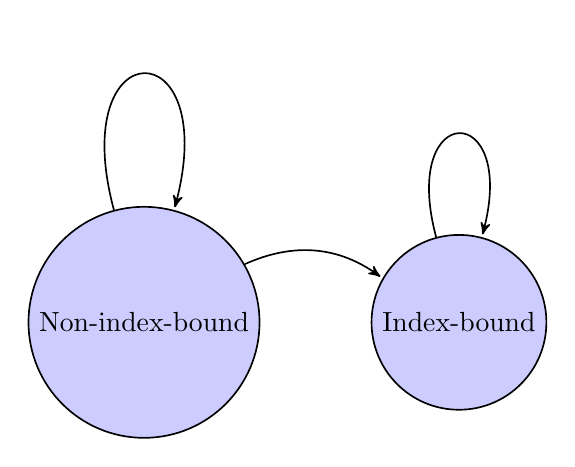
\begin{tikzpicture}[->,>=stealth',shorten >=1pt,auto,node distance=4cm, semithick]
  \tikzstyle{every state}=[fill=blue!20,draw=black,text=black]

  % Nodes
  \node[state] (I) {Non-index-bound};
  \node[state] (R) [right of=I] {Index-bound};

  % Arrows / transitions
  \path (I) edge [loop above] node {} (I);      % NIB may remain NIB
  \path (I) edge [bend left] node {} (R);       % Some NIB may become IB
  \path (R) edge [loop above] node {} (R);      % IB remains IB
\end{tikzpicture}

Currently, from Theorem 4.5, we have proven that IB lists are closed under shifts and will always permute to other IB lists. 

However, to formally show that this conceptual Markov chain is absorbing, and that any NIB list of consecutive numbers from 1 to $|L|$ will eventually become IB, we would need to prove that every NIB list is transient, permuting to an IB list after a finite number of shifts.

We now proceed to provide proofs that each support the transient property of NIB lists.

\subsubsection{Initial Proof That If NIB Lists Are Transient If It Does Not Enter A Cycle Of NIB Lists}

From Theorem 4.2, a consecutive list $L$ of length $|L|$ has $2^{|L|-1}$ possible index-bound arrangements. 

Since the set of all arrangements of $L$ can be partitioned into index-bound (IB) and non-index-bound (NIB) lists, the number of non-index-bound arrangements is simply the total number of permutations of $L$ minus the number of IB arrangements, i.e.,

\[
\text{NIB arrangements} = |L|! - 2^{|L|-1}.
\]

Since this number is finite, then if the shift sequence of an NIB list does not enter a cycle composed entirely of NIB lists, then this proves that NIB lists are transient and will eventually permute to an IB list given a finite number of shifts in numerical sorting.

Now, we will provide proof that shift sequences of NIB lists do not enter such a cycle, and eventually must permute to an IB list.

\subsubsection{Proof That A Cycle Composed Of Entirely NIB Lists Cannot Exist}

If a list L is non-index-bound, there exists an element $d_0$ at index $i_0$ where $i_0>d_0$, where $d_0>|L|$.

This is based on the given defined rules of index-bound lists where any element n in a list L where $n \leq |L|$ has to have an index i where $0 \leq i \leq n$.

Since an element in a valid list must have an index greater than zero, the existence of element $d_0$ has to hold.

Thus, a non-index-bound list can be expressed in the form $[..., d_0, ...]$, where $d_0$ is the element with the lowest index that does not satisfy IB conditions.

We can consider that if $d_0$ were to be shifted to the front, it could only shift to index $d_0$. However, we know that $i_0>d_0$. Thus, if $d_0$ were to be displaced to the left from its current index, it would be unable to return to the same index, from Theorem 3.1.

Thus, assuming that a cycling sequence composed entirely of NIB lists exists, then elements with index i where $i \geq i_0$ cannot be displaced to the left.

Therefore, in an NIB list, if an element $n$ is displaced to the first index where $n \geq i_0$, then no sequence of shifts can cycle it back to the same NIB list, because it would displace at least one element that is unable to return to the same index.

However, we can prove that within the list slice $L[:i_0]$, from the first element to the element before $d_0$, that such a number will be displaced to the first index.

To substantiate this, we will prove first that within a list slice $L[:i_0$], there exists a number $n$ where $n>i_0$, specifically in the case where $L$ is an arrangement of a consecutive list starting from 1, as it applies to our previous proofs.

\subsubsection{Proof That A List Slice $L[i_0]$ Where L Is An Arrangement Of A Consecutive List Starting From 1 Contains A Number Greater Than $i_0$}

Consider an NIB list $L$, that is an arrangement of consecutive numbers from 1 to $|L|$.

Then, there exists an element $d_0$ at index $i_0$ where $i_0>d_0$, where $d_0>|L|$.

However, one can show $d_0 \neq |L|$, the largest element in the list.

This is because the only condition for an IB list is such that every element $n$, if $n \leq |L|$, then $0 \leq i \leq n$.

However, $|L|$ will not have to satisfy the conditions because $|L|=|L|$.

Thus, $|L| > d_0$ for any given NIB list.

Now, let us consider two cases, one in which in a given NIB list the index of $|L|$ is lower than $i_0$, and the other where the index of $|L|$ is greater than $i_0$.

It is trivial to prove the statement holds for the case where the index of $|L|$ is lower than $i_0$, since the list slice $L[:i_0]$ will have to contain $|L|$ which can displace $i_0$ since $|L|>i_0$.

However, the statement is harder to prove for the case where the index of $|L|>i_0$. Since $|L|$ will not be in the list slice $L[:i_0]$, we have to prove the existence of a new element that is greater than the index $i_0$ in the list slice $L[:i_0]$.

Let us prove the existence of this element by considering the continued construction of an NIB list, attempting to break the conditions by shifting an element greater than $i_0$ behind $i_0$.

\subsubsection{Continued Proof Of 4.2.6 For When Index Of $|L| > d_0$}

Since $|L|$ is the greatest number in the list and $|L| \neq d_0$, then if $d_0$ has a greater index than $|L|$, there exists a number $(|L|)$ that is greater than $i_0$ in the list slice $L[:i_0]$.

\textbf{(Unfinished proof, work in progress! This will be updated in a future revision of this preprint.)}

\section{Theoretical Observations And Open Combinatorial Conjectures}
While we have proven that some list arrangements can be sorted using numerical sorting, there are some open conjectures that I am unable to currently prove, that may suggest other potential sortable list arrangements.

\subsection{Conjecture Of Addition}

If a positive integer $k$ is added to a consecutive list of numbers $L$ from $L[0]$ to $|L|$, then the number of shifts needed to sort $L$ is equal to:

\begin{enumerate}[start=1]
    \item $(L[0]+k+1)^{|L|-k-1}$ if $L[0]+k<|L|$
    \item $|L|$ if $L[0]+k\geq|L|-1$
\end{enumerate}

\subsection{Conjecture Of Extension}

If a positive integer $|L|+1$ is appended to a consecutive list of numbers $L$ from $L[0]$ to $|L|$, then the number of shifts needed to sort $L$ is equal to:

\begin{enumerate}[start=1]
    \item $(L[0]+1)^{|L|}$ ($|L|$ taken before appending)
\end{enumerate}

These conjectures are significant because of they are proven, it can also prove that any sequence of consecutive numbers can be sorted, and not just in the case from 1 to $|L|$.

This is because we can take the simple list, $[1,2]$, and perform the necessary extension to match any consecutive list's length, as well as the necessary addition, allowing us to get a finite number that represents the number of shifts it needs to sort. (We do not include lists of length 1, since by definition they are already sorted.)

\textbf{(Unfinished section, work in progress! More details and observations will be added to this in a future preprint to strengthen the conjectures.)}

\section{Performance Evaluation And Algorithm Optimisation}
While we have proven numerical sorting works for certain arrangements of lists, we have yet to analyse its computational complexity. This section aims to measure the performance of the algorithm as well as optimise it through empirical testing, across large input sizes.

\subsection{Time Complexity Analysis Of Numerical Sorting}

One current basic Python implementation is defined below, using list slicing to recreate the shifts in the numerical sorting algorithm.

\begin{lstlisting}[language=Python]
#Function to check if list l is sorted.
def is_sorted(l):
    for i in range(len(l)-1):
        if l[i] > l[i+1]:
            return False
    return True

#Numerical sorting function, performing shifts until l is sorted.
def sort(l):
    s = len(l)
    while True:
        n = l[0]
        if n < s:
            l = l[1:n+1] + [n] + l[n+1:]
        else:
            l = l[1:] + [n]
            if is_sorted(l):
                return l
\end{lstlisting}

Because the number of shifts varies given the nature of the list, the time complexity of the algorithm is hard to gauge from looking at the code. For example, some lists with duplicates may not even sort at all, while consecutive lists sort in a fixed number of shifts, though suggesting an exponential time complexity. ($2^{n-1}$ as shown from Theorem 4.1)

However, we can attempt to estimate the given time and space complexity of the algorithm by measuring its performance and RAM consumption by sorting different sizes of lists and taking the average of many trials.

Below is an empirical test we can perform to evaluate the algorithm's time complexity.

\subsubsection{Empirical Time Trials For Numerical Sorting And Graphical Analysis Using Matplotlib (Arrangements Of Consecutive Lists From 1 to n)}

To estimate the time complexity of numerical sorting, we first generate a series of test inputs of varying sizes.

In the following empirical test, lists where $1 \leq |L| \leq 16$ have been chosen, due to the rapid growth of shifts needed to sort lists using numerical sorting as list size grows.

We can also use the \emph{perf\_counter} function from Python's time library to measure the time taken for 10,000 sorting trials.

Assuming latency and other sources of delay are negligible, we can average these trials and plot the average time taken to sort random list arrangements against the input size.

Below is a graphical plot of the average time taken for numerical sorting to sort random arrangements of such lists across 10,000 trials, constructed by Matplotlib.

\begin{figure}[H]
    \centering
    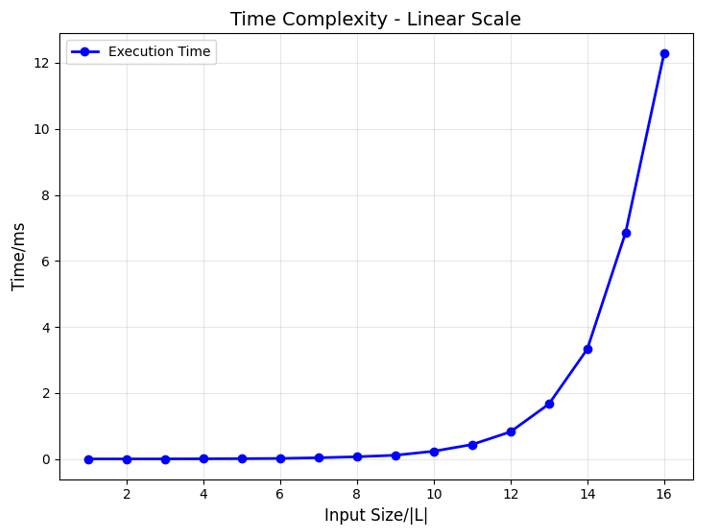
\includegraphics[width=0.75\linewidth]{Time_Complexity.png}
    \caption{Average Time Taken For Numerical Sorting In 10,000 Trials Against Input Size Of A Random Arrangement Of A Consecutive List from 1 to $|L|$}
    \label{fig:placeholder}
\end{figure}

From the graph, the empirical results indicate that the runtime of numerical sorting indeed grows at an exponential rate.

To further justify this, we can perform regression analysis by computing the coefficient of determination ($R^2$) for various candidate complexity classes using the package \emph{scipy.stats}.

Using empirical data, best-fit lines were plotted using equations derived from the following candidate complexity classes.

\begin{center}
\subsubsection{Candidate Complexity Classes}
\begin{tabular}{ll}
Linear: & $t = a|L| + b$ \\
Quadratic: & $t = a|L|^2 + b$ \\
Log-linear: & $t = a|L|\log_{10}|L| + b$ \\
Exponential: & $t = a k^{|L|}$
\end{tabular}
\end{center}

Plotting the following equations and performing regression analysis, the corresponding $R^2$ values were 0.4783, 0.6556, 0.5439, and 0.9882, respectively.

Thus, linear regression strongly supports an exponential model, with its best-fit function yielding a growth factor of $k = 1.787872$ and a base constant of $a = 8.30 \times 10^{-7}$.

In conclusion, the average time complexity of numerical sort when sorting lists that are arrangements of consecutive numbers from 1 to $|L|$ can be approximated as 
\[
O(1.79^n) \;\approx\; O(2^n).
\]

However, observe that when the input list changes, the average time complexity may be different.

This is because numerical sorting relies solely on value-based shifts rather than any fixed comparisons or list iterations. Hence, convergence patterns differ based on the input domain.

Below is the same graph of average execution time against input size for arrangements of consecutive lists without a leading 1.

While the convergence of most arrangements of consecutive lists without a leading 1 has been unproven, though IB cases are speculated to be true due to the Conjecture Of Addition, none of the lists performed in the empirical experiments failed to sort.

\begin{figure}[H]
    \centering
    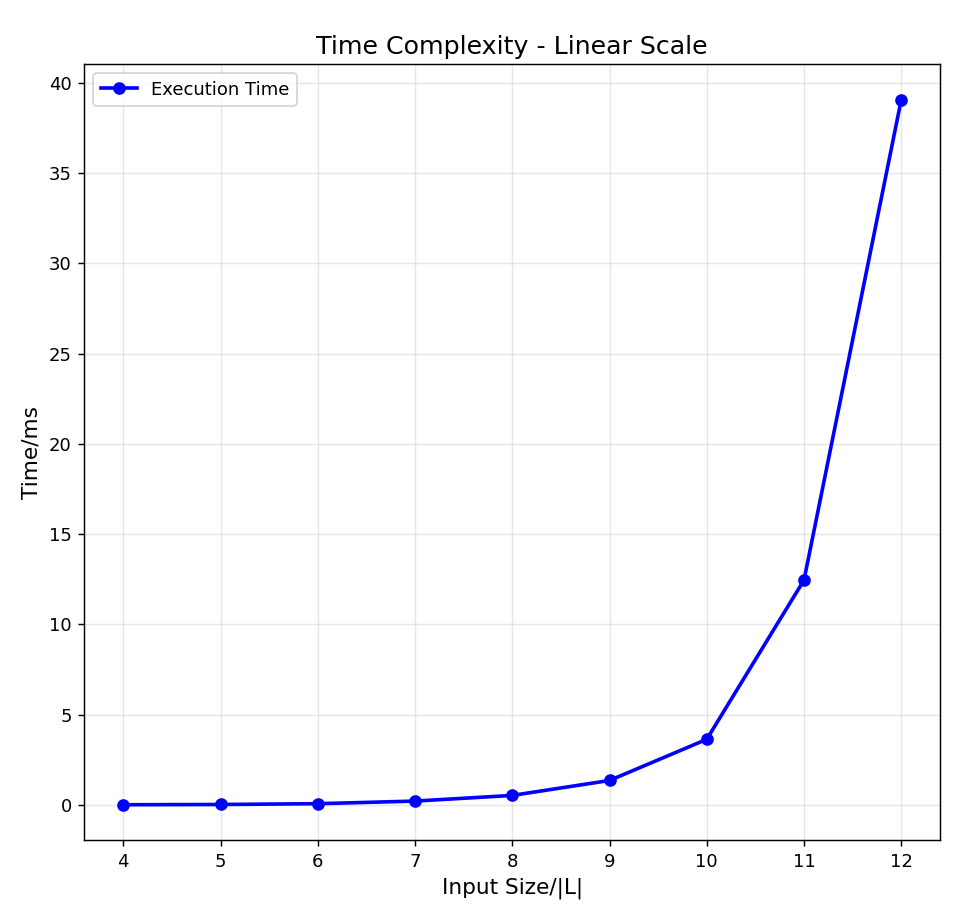
\includegraphics[width=0.75\linewidth]{Time_Complexity_2.png}
    \caption{Average Time Taken For Numerical Sorting In 10,000 Trials Against Input Size Of A Random Arrangement Of A Consecutive List from 2 to $|L|+1$}
    \label{fig:placeholder}
\end{figure}

10,000 trials were run again for each list length, with a given range of $4 \leq |L| \leq 12$, since smaller lists resulted in alternating subsequence fail cases such as in $[4,3,2]$.

Even though the exponential nature of numerical sort remains consistent, with a best-fit function of $ak^{|L|}$ having the highest coefficient of determination $R^2$ at 0.999, the function yielded a growth factor of $k=2.797111$ and a base constant of $a=1.46 \times 10^{-7}$ instead.

Hence, the empirical data for sorting consecutive list arrangements without a leading 1 suggests a time complexity of $O(2.80^n) \approx O(3^n)$, which grows much faster than the initial predicted $O(2^n)$, reflecting the speculated growth of list sorting in the Conjecture of Addition.

This suggests how numerical sort's behaviour is largely dependent on the given input list, and especially on the smallest number on the list, as well as any gaps in the range of numbers in the list.

Assuming perfect convergence and a consecutive list arrangement domain, as well the validity of the Conjecture Of Addition, then numerical sort's average time complexity can be estimated to roughly be $O((k+1)^n)$, where $k$ is the smallest number in the list.

\subsection{Space Complexity Analysis Of Numerical Sorting Implementations And Suggested Optimisations}

As stated before, the current Python implementation that has been used for testing is as written below.

\begin{lstlisting}[language=Python]
#Function to check if list l is sorted.
def is_sorted(l):
    for i in range(len(l)-1):
        if l[i] > l[i+1]:
            return False
    return True

#Numerical sorting function, performing shifts until l is sorted.
def sort(l):
    s = len(l)
    while True:
        n = l[0]
        if n < s:
            l = l[1:n+1] + [n] + l[n+1:]
        else:
            l = l[1:] + [n]
            if is_sorted(l):
                return l
\end{lstlisting}

While this specific implementation of the algorithm works, its space complexity is far from ideal because each list slice used when performing a shift is stored directly in memory and can lead to rapid RAM consumption.

In the best case, it is $O(n)$ depending on the speed of Python's garbage collection, a built-in automatic memory management system that reclaims memory occupied by objects no longer in use by the program.

Meanwhile, in the worst case, the space complexity of this implementation of the algorithm could be $O(kn)$, where $k$ is the number of shifts needed to sort the given list.

We can verify this using the \emph{tracemalloc} module in Python, and graphing memory use against the same input sizes used in Figure 1.

\begin{figure}[H]
    \centering
    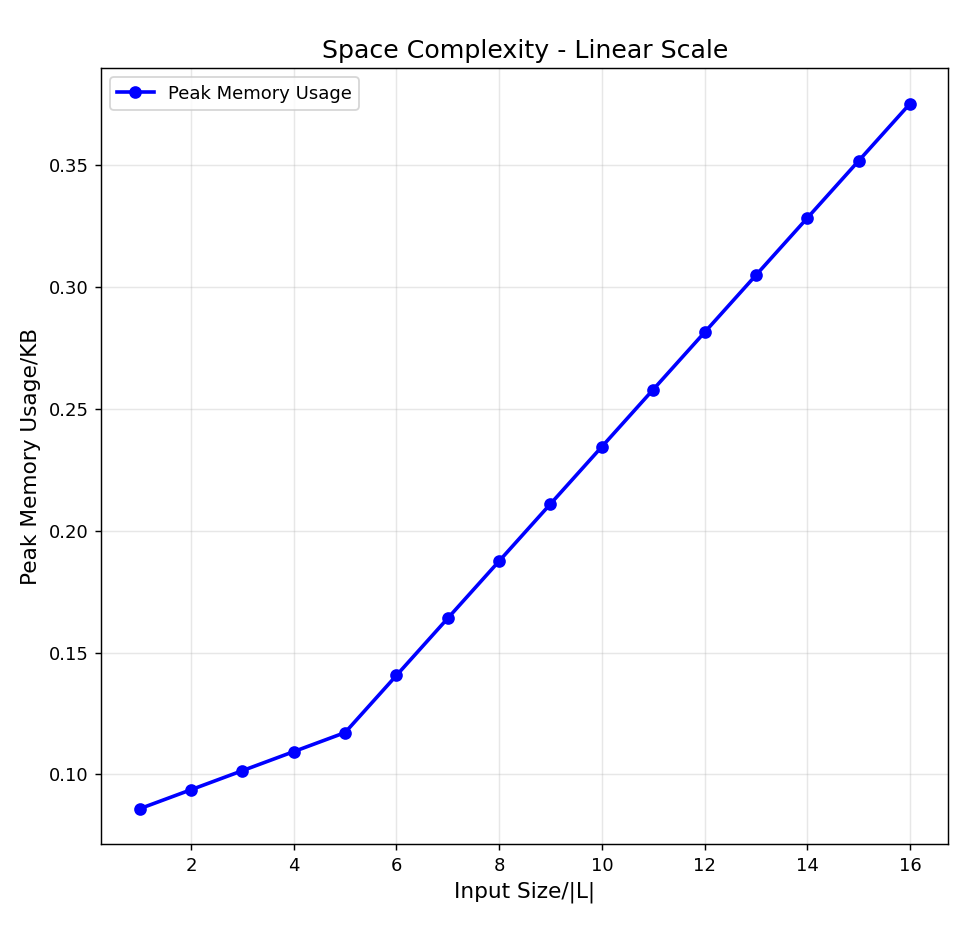
\includegraphics[width=0.75\linewidth]{Space_Complexity.png}
    \caption{Enter Caption}
    \label{fig:placeholder}
\end{figure}

As can be observed from the graph, the peak memory usage consumed during numerical sort increases in a linear trend.

However, it appears that in lists from length 1 to 5, the rate of growth in memory consumption is slower than with lists of greater length.

Therefore, the largest coefficient of determination given by the four best-fit complexity classes in 6.1.2 actually show that a log-linear best represents the given output in this input domain, with a coefficient of determination of $R^2=0.9965$, compared to that of the best-fit linear function which returned a coefficient of determination of $R^2=0.9809$.

Given the exponential nature of numerical sort, it is computationally expensive to extend the input domain due to the rapid growth in execution time. However, given what we know from the code, an $O(n)$ space complexity is more likely than an $O(nlogn)$ space complexity due to larger list slices being stored in memory as the length of the input list increases.

\subsubsection{Numerical Sort Memory Optimisation Using Insert And Pop}

To increase efficiency of memory usage, we can remove the use of list slicing to perform shifts and instead use Python's \emph{insert} and \emph{pop} to simulate a shift by inserting the first element at the correct place, before subsequently deleting it.

\begin{lstlisting}[language=Python]
#Function to check if list l is sorted.
def is_sorted(l):
    for i in range(len(l)-1):
        if l[i] > l[i+1]:
            return False
    return True

#Numerical sorting function, performing shifts until l is sorted.
def sort(l):
    s = len(l)
    while True:
        n = l[0]
        if n < s:
            l.insert(n+1, n)
            l.pop(0)
        else:
            l.insert(s, n)
            l.pop(0)
            if is_sorted(l):
                return l
\end{lstlisting}

With this implementation of the algorithm, we run the same empirical tests on memory usage across trials of different input sizes.

\textbf{(Unfinished empirical tests, work in progress! The graph for the memory performance of this improved implementation will be added in a future version of the preprint.)}

\subsection{Potential Reduction To Polynomial Time Using Different Shift Rules}

From our previous findings, numerical sort tends to have exponential time complexity on average, with execution time growing rapidly as the size of input lists increases.

This makes it unpractical and computationally expensive for larger lists, since it will perform huge numbers of operations just to sort small-order lists.

However, we can attempt to reduce it to polynomial time by changing shift rules, and adjusting algorithmic steps.

One inefficient behaviour of numerical sorting that can be observed is how it tends to exhibit recursion, that can be re-observed in the simple case of the sorting of the list $[1,2,3,4,5]$.

\subsubsection{Shift Sequence Of A Length-5 Consecutive List}
\begin{enumerate}[start=0]
    \item $[1, 2, 3, 4, 5]$
    \item $[2, 1, 3, 4, 5]$ (1 has to be displaced before 3 is displaced)
    \item $[1, 3, 2, 4, 5]$
    \item $[3, 1, 2, 4, 5]$ (2, 1 has to be displaced before 3 is displaced)
    \item $[1, 2, 4, 3, 5]$
    \item $[2, 1, 4, 3, 5]$
    \item $[1, 4, 2, 3, 5]$
    \item $[4, 1, 2, 3, 5]$ (3, 1, 2 has to be displaced before 4 is displaced)
    \item $[1, 2, 3, 5, 4]$
    \item $[2, 1, 3, 5, 4]$
    \item $[1, 3, 2, 5, 4]$
    \item $[3, 1, 2, 5, 4]$
    \item $[1, 2, 5, 3, 4]$
    \item $[2, 1, 5, 3, 4]$
    \item $[1, 5, 2, 3, 4]$
    \item $[5, 1, 2, 3, 4]$ (4, 1, 2, 3 has to be displaced before 5 is displaced)
    \item $[1, 2, 3, 4, 5]$
\end{enumerate}

In this specific example, notice how 2 needs 1 to displace it, 3 needs 2 and 1 to displace it, 4 needs 3, 2, and 1 to displace it, and 5 needs all four other numbers to displace it.

This can be observed by viewing the first number of intervals when 1 is displaced to the front, to when 2 is displaced to the front, 3, and so on.

Because the program has to displace an increasingly larger number of numbers to displace the next number, the number of required operations grows exponentially.

However, one can observe that in this example, after a number $n$ shifts to an index directly after $n+1$ and decreases $n+1$'s index, the next step is usually to bring $n+1$ to the front index.

Then, we can optimise the efficiency of the algorithm so that after a shift, it directly shifts the element before it to the front index.

This means that with a list $[n, a_1, a_2, ..., a_n]$, $n$ shifts forward to $[a_1, a_2, ..., a_n, n]$, and then brings its previous element to the front index to permute the list to $[a_n, a_1, a_2, ...,n]$.

This is also equivalent to swapping the element at index 0 and index $n$, since the element at index 0 will increase to index $n+1$, and the previous element at index $n$ will be shifted to index 0, and thus the element at index $n+1$ will fall to index $n$.

However, if $L[0]\geq|L|$, then there is no element at index $L[0]+1$ to swap, since it would be greater than the length of the list.

One possible approach is to swap $L[0]$ with the element at index $|L|-1$, however this may give rise to fail cases because swapping fails to sort the list when two values are greater or equal to $|L|-1$, such as in $[5,1,2,3,4]$, since swapping will cause a cycling sequence of $[4,1,2,3,5]$ and back to $[5,1,2,3,4]$.

Instead, we can make such elements shift directly to the back, following the previous algorithmic rules of numerical sort, and avoiding this fail case.

Therefore, we can now define a new sorting algorithm borrowing from the value-based approach of numerical sort.

Let us define this new algorithm as swap sort, with the given rules below.

\subsection*{Swap Definition}

\begin{itemize}
    \item Take the first element $n = L[0]$.
    \item If $n < |L|$, swap $L[0]$ with $L[n]$.
    \item Otherwise, move $n$ to the end of the list.
\end{itemize}

Formally, the swap can be described as the following.
\[
\text{shift}(L) = 
\begin{cases}
L[n] \| L[1:n] \| [L[0]] \| L[n+1:] & \text{if } n < |L|\\
L[1:] \| [L[0]] & \text{otherwise}
\end{cases}
\]

\subsection*{Python Implementation}
\begin{lstlisting}[language=Python]
#Function to check if list l is sorted.
def is_sorted(l):
    for i in range(len(l)-1):
        if l[i] > l[i+1]:
            return False
    return True

#Swap sorting function, performing swaps/shifts until l is sorted.
def sort(l):
    s = len(l)
    while True:
        n = l[0]
        if n < s:
            l[0], l[n] = l[n], l[0]
        else:
            l.pop(0)
            l.append(n)
            if is_sorted(l):
                return l
\end{lstlisting}

While swap sort is based on current observations from numerical sorting patterns, we have yet to formally prove that it can sort the same given input domain of lists (consecutive list arrangements from 1 to $|L|$).

Let us provide some proofs that swap sort can sort IB lists that are arrangements of consecutive lists from 1 to $|L|$, and prove that NIB lists always permute to IB lists in swap sort.

\subsubsection{Proof That Swap Sort Permutes An IB List To Another IB List}
First, we can prove that when a swap is performed on an IB list, it will always permute to another IB list.

This is because assuming an IB list already satisfies the conditions where every element in which $k < |L|$ satisfies $0 \leq i \leq k$, then swapping the element at index $n$ to index 0 will not change the statement that $0 \leq i \leq L[n]$, since its new index will be 0, satisfying the condition.

Meanwhile, since the element $L[0]$ initially at index 0 will have a new index of $L[0]-1$, where $0 \leq L[0]-1 \leq L[0]$, then it will also satisfy IB conditions.

Finally, since we have also previously proven that moving $L[0]$ to the back of the list in the case where $L[0] \geq |L|$ also results in an IB list in Case 1 of 4.2.2, then we have proven that the swap sort algorithm will always permute an IB list to an IB list with one swap/shift.

Thus, we can state the following theorem.

\begin{theorem}
 All index-bound lists will permute to only index-bound lists after a swap operation in swap sort.
\end{theorem}

\subsubsection{Proof That IB Lists That Are Consecutive List Arrangements From 1 to $|L|$ Will Always Sort In Swap Sort}

To prove that IB lists that are consecutive list arrangements from 1 to $|L|$ will always sort in swap sort, let us consider the chain of events that result from swapping in swap sort.

First, let a list $L = [a_1,a_2,a_3,...]$.

Then, we can consider the following first elements of the list after a swap.

Since a swap either swaps $L[0]$ and $L[L[0]]$ or shifts $L[0]$ to the back, a chain reaction will continue where a swap leads to another swap, i.e.

\[
\text{L[0] sequence} = a_1 \rightarrow L[a_1] \rightarrow L[L[a_1]] \rightarrow L[L[L[a_1]]] \dots
\]

Eventually, this chain will lead to the displacement of an element to the first index where $L[0] \geq |L|$.

This is because the sequence cannot repeat, as after a swap where an element $i$ swaps with $L[i]$, then the only element that could swap to $L[i]$ will be $L[i]$, which cannot be swapped back to the first index, since there are no duplicates in an arrangement of a consecutive list of 1 to $|L|$.

With a finite number of IB list arrangements of consecutive numbers from 1 to $|L|$ equal to $2^{n-1}$, then the chain will eventually displace an element to the first index where $L[0] \geq |L|$.

This is important because we know that the only element in a consecutive list arrangement from 1 to $|L|$ that is greater or equal to $|L|$ will be $|L|$.

We also know that this will have to be an IB list according to Theorem 5.1, where $|L|=L[0]$. However, this list is necessarily equal to $[|L|, 1, 2, ..., |L|-1]$, since by IB list conditions, 1's index has to be within zero and one.

Thus, it has to be placed at index one. But this leaves 2 with only index 2 where $0 \leq i \leq 2$, which also leaves 3 with only index 3 where $0 \leq i \leq 3$, and so on for greater numbers.

Therefore, the only IB list arrangement where $|L|=L[0]$ is equal to $[|L|, 1, 2, ..., |L|-1]$. Finally, we can easily show that in one operation, swap sort can sort it, because given the rules where $L[0] \geq |L|$, it will be shifted to the back.

This permutes the list $[|L|, 1, 2, ..., |L|-1]$ to $[1, 2, ..., |L|-1, |L|]$, sorting the list.

Ultimately, since an IB list that is a consecutive list arrangement from 1 to $|L|$ will undergo a sequence of swaps that eventually end in $L[0]=|L|$, which is guaranteed to be sorted in another operation, then all IB lists that are consecutive list arrangements from 1 to $|L|$ will eventually be sorted using the swap sort algorithm.

Therefore, we have proven that the swap sort algorithm works for this case, and can summarise the previous findings as the following theorems and corollaries.

\begin{theorem}
 For an arrangement of a consecutive list (1 to $|L|$), $|L|$ will be swapped to the first index after a finite number of swaps.
\end{theorem}

\begin{theorem}
 The only IB arrangement of a consecutive list from 1 to $|L|$, where $L[0]=|L|$, can be expressed as the form $[|L|,1,2,...,|L|-1]$
\end{theorem}

\begin{corollary}
 All index-bound arrangements of consecutive lists (1 to $|L|$) can be sorted using swap sorting.
\end{corollary}

\subsubsection{Proof That NIB Lists Will Always Permute To IB Lists And Thus Will Sort Using Swap Sort}

First, let us consider the sequence of swaps that arises from the swap sort algorithm.

\[
\text{L[0] sequence} = a_1 \rightarrow L[a_1] \rightarrow L[L[a_1]] \rightarrow L[L[L[a_1]]] \dots
\]

\textbf{(Unfinished proof, work in progress! This will be updated in a future revision of this preprint.)}

\subsection{Swap Sort Time Complexity Analysis}

Now that we have proven that swap sort works for all consecutive list arrangements from 1 to $|L|$, we can perform similar empirical testing to estimate the time complexity of the algorithm.

Given that the algorithm now heavily relies on efficient item assignment through swaps instead of rapid popping and inserting of list elements, it is likely that time complexity has been massively improved, alongside the transformation of the recursive nature of the algorithm.

Below is a graph of the average execution time of 10,000 trials of swap sort from input sizes of 1 to 1024, with an interval of 1.

\begin{figure}[H]
    \centering
    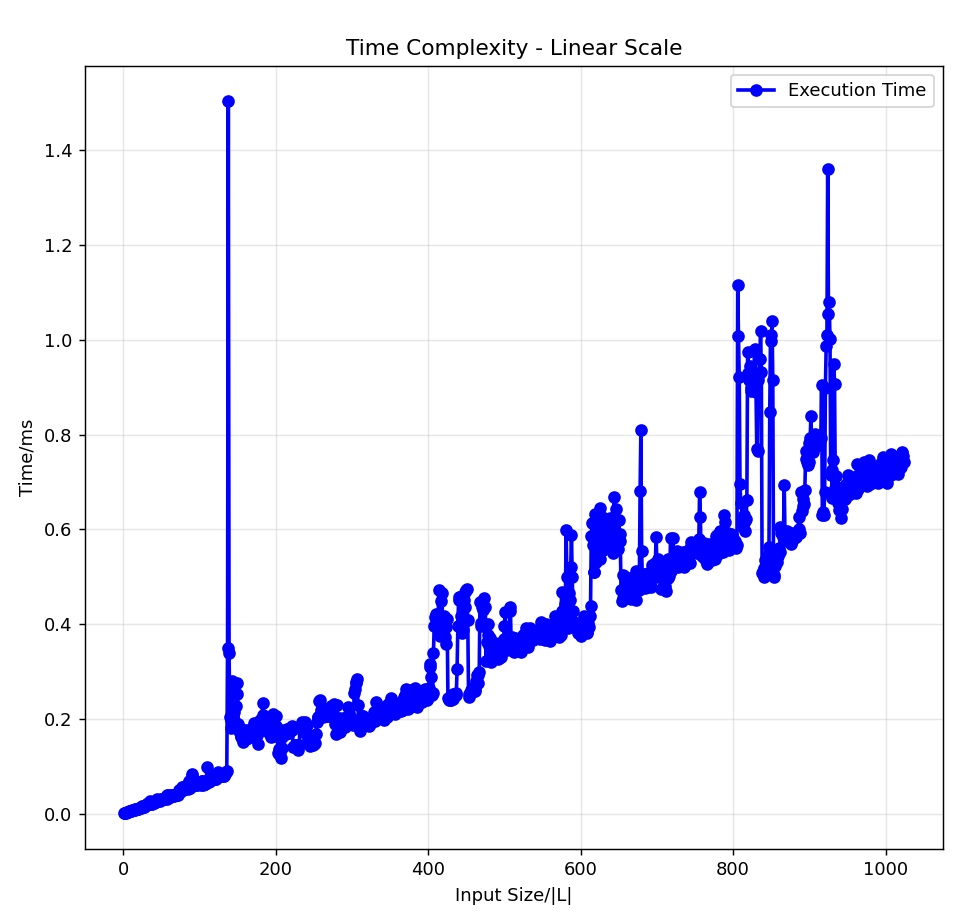
\includegraphics[width=0.75\linewidth]{Time_Complexity_Swap.png}
    \caption{Average Time Taken For Swap Sort In 10,000 Trials Against Input Size Of A Random Arrangement Of A Consecutive List from 1 to $|L|$}
    \label{fig:placeholder}
\end{figure}

Again, the swap sorting algorithm appears to not follow a fixed time complexity, with some significant outliers in the data such as with lists of size 138, taking after 1.50ms on average to sort.

However, by approximating best-fit functions with the same four complexity classes as mentioned in 6.1.2, the closest fit appears to be either a linear or log-linear function, with a coefficient of determination of $R^2=0.8571$ and $R^2=0.8569$ respectively.

This hence suggests that for the given input domain of consecutive list arrangements from 1 to $|L|$, the average time complexity of swap sort is around $O(n)$, though $O(nlogn)$ is also a decent candidate due to the small percentage difference between the two coefficients of determination.

This is a marked improvement of roughly $O(2^n)$ time complexity in numerical sort versus $O(n)$ in swap sort, which has effectively reduced the time complexity from exponential to polynomial time.

\subsection{Swap Sort Space Complexity Analysis}
Like the previous improvement in numerical sort, the new algorithm of swap sort also benefits from $O(1)$ space complexity.

This is because the only necessary items stored in memory during swap sort are simple variables that point to $L[0]$ and $L[L[0]]$.

\section{Benchmark Tests With Other Sorting Algorithms}

Now that we have markedly improved our value-based shifting algorithm from $O(2^n)$ time complexity in numerical sort to $O(n)$ in swap sort with $O(1)$ space complexity, we can benchmark swap sort with other common and popular examples of sorting algorithms on time and memory usage.

In the following empirical tests, I benchmarked swap sort on average execution time and peak memory usage with the following 10 other sorting algorithms.

\subsubsection{Benchmark Sorting Algorithms}

\begin{enumerate}[start=1]
    \item \textbf{Quicksort} - A divide-and-conquer algorithm that selects a pivot element and partitions the list into elements smaller and larger than the pivot, then recursively sorts the partitions. Average time complexity: O(n log n), worst case: O(n²). Space complexity: O(log n) average, O(n) worst case.
    
    \item \textbf{Merge Sort} - A stable divide-and-conquer algorithm that recursively divides the list into halves, sorts each half, then merges the sorted halves back together. Time complexity: O(n log n) in all cases. Space complexity: O(n).
    
    \item \textbf{Heap Sort} - Uses a binary heap data structure to repeatedly extract the maximum (or minimum) element and place it at the end of the sorted portion. Time complexity: O(n log n) in all cases. Space complexity: O(1).
    
    \item \textbf{Insertion Sort} - Builds the sorted list one element at a time by inserting each element into its correct position among the previously sorted elements. Time complexity: O(n²) worst and average case, O(n) best case. Space complexity: O(1).
    
    \item \textbf{Selection Sort} - Repeatedly finds the minimum element from the unsorted portion and moves it to the beginning of the sorted portion. Time complexity: O(n²) in all cases. Space complexity: O(1).
    
    \item \textbf{Shell Sort} - An extension of insertion sort that allows the exchange of items that are far apart, gradually reducing the gap between compared elements. Time complexity depends on gap sequence, typically $O(n \log^2 n)$ to $O(n^{3/2})$. Space complexity: O(1).
    
    \item \textbf{Radix Sort} - A non-comparative sorting algorithm that sorts integers by processing individual digits, starting from the least significant digit. Time complexity: O(d × n) where d is the number of digits. Space complexity: O(n + k) where k is the range of digits.
    
    \item \textbf{Bubble Sort} - Repeatedly steps through the list, compares adjacent elements, and swaps them if they are in the wrong order. Time complexity: O(n²) worst and average case, O(n) best case. Space complexity: O(1).
    
    \item \textbf{Counting Sort} - A non-comparative sorting algorithm that counts the occurrences of each distinct element and uses this information to place elements in their correct positions. Time complexity: O(n + k) where k is the range of input. Space complexity: O(k).
    
    \item \textbf{Cycle Sort} - An in-place sorting algorithm that minimizes the number of memory writes by placing each element directly into its final position through a series of cycles. Time complexity: O(n²). Space complexity: O(1).
\end{enumerate}

To benchmark each of the sorting algorithms, we generate consecutive list arrangements from 1 to $|L|$, from $200 \leq L \leq 2000$, with an interval of 200.

Five trials were performed for each sorting algorithm, and the average was taken.

Below are the results of plotting average execution time in seconds against input size.

\begin{figure}[H]
    \centering
    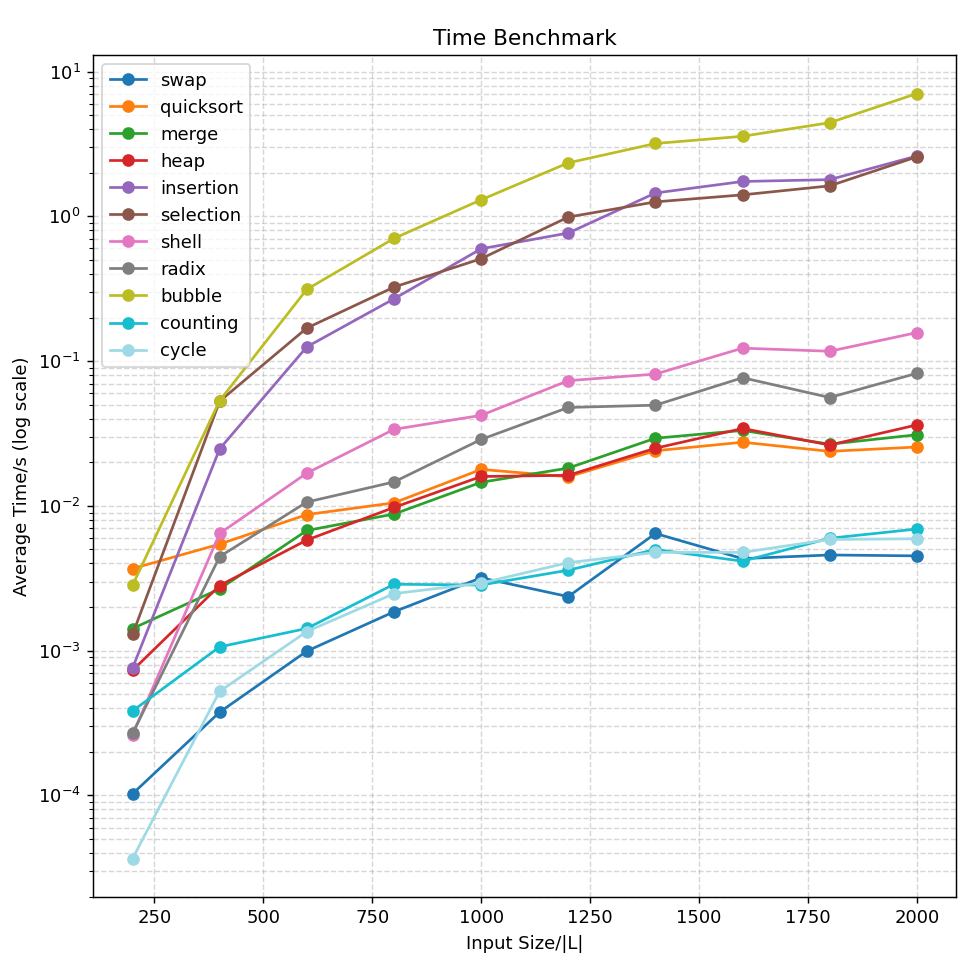
\includegraphics[width=0.75\linewidth]{Time_Benchmark.png}
    \caption{Average Time Taken For Swap Sort And 10 Other Sorting Algorithms In 5 Trials Against Input Size Of A Random Arrangement Of A Consecutive List from 1 to $|L|$}
    \label{fig:placeholder}
\end{figure}

From the graph, we can see that bubble sort performs the worst on time, which is expected due to its $O(n^2)$ time complexity, as it compares individual elements in the list.

This is followed by insertion and selection sort which both closely approach $O(n^2)$ time complexity.

With much faster performance, we then have shell and radix sort which both have unique time complexities at roughly $O(n \log^2 n)$ to $O(n^{3/2})$, and $O(d \times n)$ where $d$ is the number of digits, which is $3-4$ in the given input domain.

After that, we have merge, heap, and quicksort which perform decently well at log-linear time complexities of $O(nlogn)$, with similar execution times on average.

However, the empirical data shows the best sorting algorithms based on fastest execution time with the given domain would be counting sort, cycle sort, and swap sort, nearing $O(n)$ time complexity.

Meanwhile, tracking the peak memory usage in kilobytes of the same sorting algorithms with the same given input sizes, below are the graphs of peak memory usage against input size.

\begin{figure}[H]
    \centering
    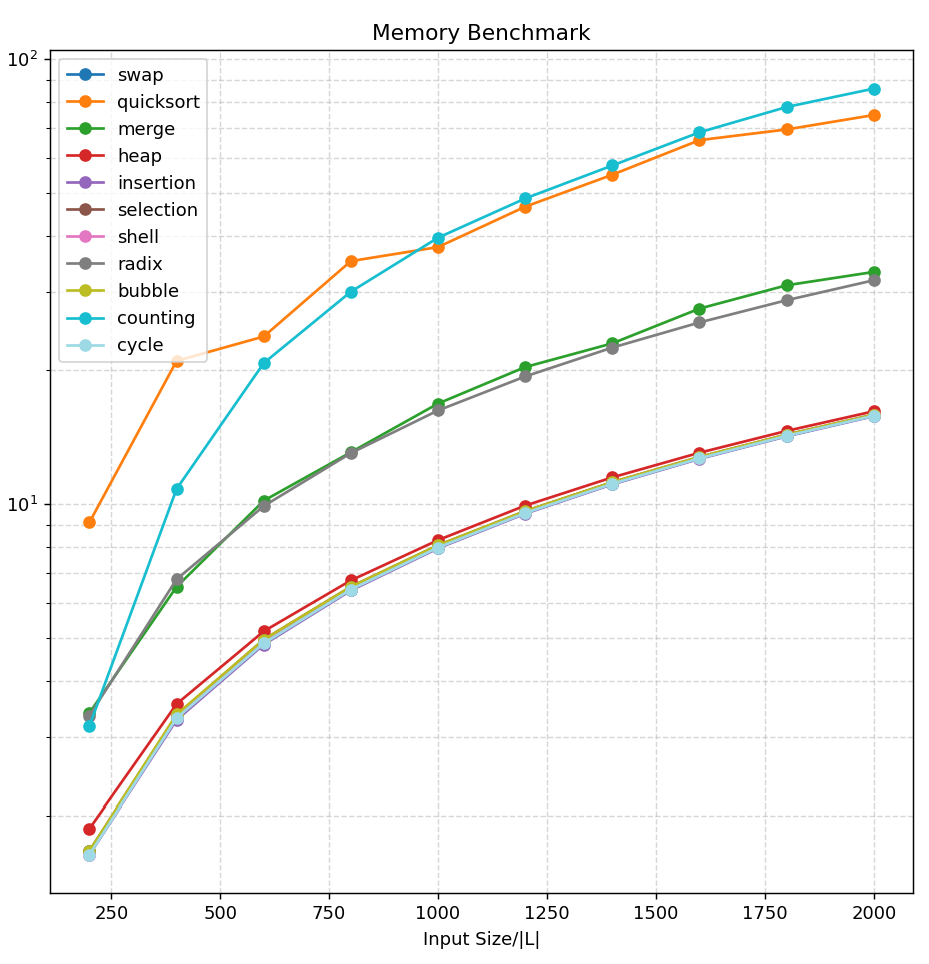
\includegraphics[width=0.75\linewidth]{Memory_Benchmark.png}
    \caption{Peak Memory Usage Of Swap Sort And 10 Other Sorting Algorithms In 5 Trials Against Input Size Of A Random Arrangement Of A Consecutive List from 1 to $|L|$}
    \label{fig:placeholder}
\end{figure}

The empirical results of peak memory usage reveal three distinct performance classes of memory consumption among the 11 sorting algorithms.

Quicksort and Counting Sort exhibit the highest peak memory usage, with Quicksort requiring substantial memory for recursive call stacks and temporary sublists during partitioning, while Counting Sort allocates auxiliary lists proportional to the input range.

This is followed by Merge Sort and Radix Sort, with lower memory demands, as Merge Sort needs $O(n)$ auxiliary space for merging operations, and Radix Sort requires temporary lists for digit-based redistribution.

Finally, the empirical data suggests the most memory-efficient algorithms include heap sort, insertion sort, selection sort, shell sort, bubble sort, swap sort, and cycle sort, all of which operate in-place with O(1) auxiliary space complexity, working with direct element manipulation without requiring significant additional storage.

While swap sort shows highly impressive results in these benchmark tests, surpassing all ten other sorting algorithms on the biggest input size in terms of average execution time, it is likely that counting and cycle sort perform better as the order of magnitude of input size increases, due to their fixed efficiency.

Additionally, while swap sort also has lightweight memory demands, the same applies to many other sorting algorithms which use direct element manipulation to sort lists instead of creating sublists or allocating memory to other needs.

Finally, one also has to factor in that swap sort is proven to work only specifically for this input domain, and swap sort may fail in other cases that extend beyond the boundaries of the paper. In those cases, other sorting algorithms are much more suited to sort them.

Hence, further mathematical characterisation and optimisation is needed to support the practical use of value-based shift algorithms as a computational model.

\section{Theoretical Discussion}
The sorting process of numerical and swap sort avoids element-wise comparisons and traditional iteration. However, their performance often acts unpredictably in time complexity due to the nature of using values for sorting instead of rigid comparisons. In some edge cases, it may take many shifts to reach a sorted state. Further mathematical characterization is needed.

\section{Conclusion}
These shift-based sorting algorithms introduce an unconventional perspective on sorting by removing the need for comparison and list iteration. While primarily a proof-of-concept, it opens a path for further study into value-guided transformations as a computational model.

(References in progress, not properly tagged yet!)
\bibliographystyle{plain}
\begin{thebibliography}{1}

\bibitem{knuth1998}
Donald E. Knuth,
\textit{The Art of Computer Programming, Vol. 3: Sorting and Searching}.
Addison-Wesley, 1998.

\end{thebibliography}

\end{document}
